\chapter{Marco Teórico} % con la palabra capitulo
%\addcontentsline{toc}{chapter}{Capítulo 2: Marco Teórico} % si queremos que aparezca en el Í­ndice
%\markboth{Capítulo 2: Marco Teórico}{Capítulo 2: Marco Teórico} % encabezado
\graphicspath{./imagenes}

En éste capítulo se muestra un ejemplo de un diagrama en la Figura \ref{fig:diagrama}
\begin{figure}[hbtp]
\scalebox{0.6}{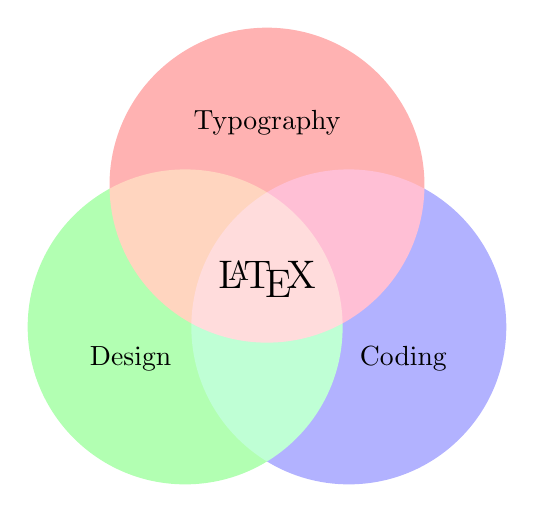
\begin{tikzpicture}
  \begin{scope}[blend group = soft light]
    \fill[red!30!white]   ( 90:1.2) circle (2);
    \fill[green!30!white] (210:1.2) circle (2);
    \fill[blue!30!white]  (330:1.2) circle (2);
  \end{scope}
  \node at ( 90:2)    {Typography};
  \node at ( 210:2)   {Design};
  \node at ( 330:2)   {Coding};
  \node [font=\Large] {\LaTeX};
\end{tikzpicture}}
\caption{Ejemplo de diagrama.}
\label{fig:diagrama}
\end{figure}
\clearpage%

